\chapter{SSAN一致性问题}

\section{原理}

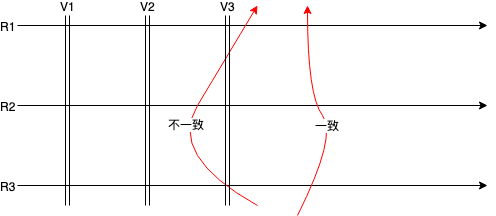
\includegraphics[width=11cm]{../imgs/consistency-splice.png}

从逻辑上讲,一致性是由任一对象的变更历史决定的。任一对象的多个副本/分片,可以看作有限状态机,
须按同一顺序执行变更。变更通常包括写IO和修复IO。

相比于副本机制,EC的各分片具有严格顺序。

从实现机制上来看,副本或EC的一致性,需要从\hl{对象版本、控制器和日志}几个方面来考虑。

恢复过程的关键是\hl{选择到正确的副本/分片}。分为几种情况:
\begin{enumbox}
\item EC的节点故障
\item EC的磁盘故障
\item 副本
\end{enumbox}

\section{EC一致性}

\subsection{对象版本}

从概念上来说,SSAN按epoch组织对象,节点故障时提升epoch,磁盘故障时epoch不变,
通过强制升级epoch来模拟节点/磁盘混合故障。

epoch是集群级别的版本,epoch内节点成员关系不变。在SSAN实现里epoch被用作粗粒度的对象版本。

\subsection{控制器}

IO控制器是gateway,SSAN原始实现无恢复控制器,后针对任一对象引入primary数据分片作为恢复控制器。
这样就形成\hl{IO和恢复的双控架构},为了对象一致性,需要同步IO控制器和恢复控制器。

\subsection{日志}

无日志,难以处理特定情况下的恢复问题。

\subsection{对象组织及其cache}

因为可能在工作目录创建不同epoch的对象,工作目录下的对象名字也要包括epoch。

进一步可以考虑按epoch组织目录,这样可以简化关键操作,比如消除rename和link操作。

维护磁盘对象结构的内存cache,在其上面提供API,合并stale cache和object list cache。

\subsection{恢复实例}

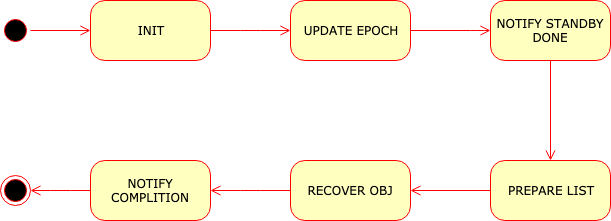
\includegraphics[width=11cm]{../imgs/recovery-fsm.png}

恢复实例可以看作有限状态机。在恢复期间,SSAN进程运行一个恢复实例。
如果有新的故障,则执行上下文切换,切换到下一恢复实例。需要保证切换恢复实例过程的正确性。
任一时刻,最多有一个恢复实例在运行。

恢复状态机的每步转换都要满足safety和liveness条件,特别需要注意的是:
\begin{enumbox}
\item update epoch过程务必成功执行
\item 若一节点收不到recover peer,无法进入NOTIFY STANDBY DONE状态
\end{enumbox}

\section{EC一致性改进之处}

具体见git仓库的提交日志。

\subsection{增强系统可追踪性}

主要通过日志机制来实现。把每个对象、io、恢复实例等等实体看作对象,追踪其生命周期行为,便于分析异常现象。

\subsection{改进对象组织方式}

\subsection{改进stale object cache}

改进stale object cache模块,用于追踪对象在磁盘上的分布,可以理解为磁盘目录结构的cache。
通过支持所需API,来替代原来的object list cache和stale cache。同时也方便stale object的GC过程。

\subsection{恢复状态机引入新状态}

引入RW\_INIT:为了实现没有进入prepare状态的恢复实例,可以切换到下一实例。一旦进入prepare阶段,则切换过程有所不同。
\hl{通用原则是确保rinfo上下文信息的安全性}。在有引用计数的情况下,不能被free掉。

引入RW\_UPDATE\_EPOCH:因为update epoch执行时间过长,为了不堵塞main线程,须放到工作线程中去做。

引入RW\_NOTIFY\_STANDBY\_DONE:放入同步点,以确保object list cache准备妥当,才能保证后续prepare object list过程无误。

避免prepare object list重复入队,导致修复崩溃

\subsection{磁盘空间不足时的恢复过程}

\todo{磁盘空间不足时的恢复过程}

\subsection{retry机制}

retry机制的使用需要具体分析,内部过程慎用retry,避免堵塞main线程,使系统失去响应能力。

重试次数和timeout值的选择也影响到故障切换时长和IO中断时长。

\subsection{Too many open files}

文件句柄数量控制,由最大1024改为1048576。直接在SSAN进程内设定。

\section{副本一致性}

现象:观察到恢复完成后,有时vdi对象并不一致。

\todo{副本一致性}目前副本的一致性实现,机制上恐有问题。
恢复的选择步骤,各个副本独立运行选择过程,所依据的并非该对象各个副本的全局信息,而是相当局部的信息。
并不能保证一定选择到正确副本。

需要参考EC一致性的机制,选出primary协调IO和recovery活动。
副本的选择步骤相对简单:可用的最大版本的副本,以之为权威副本,覆盖其余。

\section{小结}

指导原则
\begin{enumbox}
\item 一致性问题要对标相关参考模型
\item 采用流体动力学模型分析性能瓶颈
\item 工欲善其事必先利其器
\end{enumbox}

工具方面
\begin{enumbox}
\item 完整日志追踪系统,细粒度地追踪程序运行时行为
\item 多用断言,以捕获程序中的不变式,尽早暴露问题
\item 生成COREDUMP
\item 采用valgrind分析内存问题
\item 尽量配备可用的开发和测试环境
\end{enumbox}

关于日志子系统,需要进一步规范化。
